\ChapterImageStar[cap:revisionLiteratura]{Revisión sistemática de la literatura}{./images/fondo.png}\label{cap:revisionLiteratura}
\mbox{}\\
\noindent
Con el fin de fundamentar la investigación, se realizó un mapeo sistemático de estudios (\SMS). Este consistió en la búsqueda, filtrado, selección y análisis de literatura académica, artículos técnicos y reportes de caso relacionados con las \VBC. El objetivo fue obtener una visión global y estructurada sobre las tecnologías disponibles, sus tendencias de adopción y las principales dimensiones de análisis empleadas en la comunidad científica y profesional.
\section{Construcción de la bitácora}
\noindent
En búsqueda de una base teórica para la elección de una tecnología de virtualización basada en contenedores, 
se realizó una revisión del estado del arte. Esta revisión se completó en diferentes etapas:

\subsection{Planeación}
\noindent
Esta etapa consistió en establecer el propósito general que se buscaba alcanzar con el \SMS\ (\textit{Systematic Mapping Study}). 
A su vez, definió aspectos como objetivos, preguntas de investigación y métricas ver cuadros~\ref{tab:metricas},~\ref{tab:metas} y~\ref{tab:preguntas} respectivamente. Para ello, se siguió el modelo 
Objetivo-Pregunta-Métrica (\textit{Goal-Question-Metric}, GQM). A continuación, se definen los objetivos del \SMS\ aplicado 
a las tecnologías de virtualización basadas en contenedores en el cuadro.

\subsubsection{Definición de metas para el \SMS}

\begin{table}[H]
\centering
\renewcommand{\arraystretch}{1.2} % Espaciado reducido
\footnotesize % Texto más pequeño
\begin{tabular}{|c|p{13cm}|}  % Columna más ancha (12cm)
\hline
\textbf{Meta} & \textbf{Descripción} \\ \hline
G1 & Identificar trabajos relacionados de \VBC\ en docencia, investigación y extensión. \\ \hline
G2 & Clasificar trabajos relacionados de \VBC\ en dominios de \TI: desarrollo software, pensamiento computacional, computación paralela, análisis datos, IA, redes, infraestructura \TI, HPC, etc. \\ \hline
\end{tabular}
\caption{Definición de metas del SMS}
\label{tab:metas}
\end{table}

\subsubsection{Definición de preguntas de investigación}
\begin{table}[H]
\centering
\renewcommand{\arraystretch}{1.2} % Espaciado reducido
\scriptsize % Texto más pequeño
\begin{tabular}{|c|c|p{6cm}|p{6cm}|} % Columnas más estrechas
\hline
\textbf{Meta} & \textbf{Pregunta} & \textbf{Descripción} & \textbf{Motivación} \\ \hline
G1 & Q1 &
\textit{¿Cuáles trabajos de \VBC\ impactan positivamente en docencia, investigación y extensión?} &
La \VBC\ ofrece transversalidad y reproducibilidad, facilitando transporte de soluciones TI entre dominios. \\ \hline

G2 & Q2 &
\textit{¿Cuáles trabajos de \VBC\ contribuyen en dominios de \TI?} &
Proporcionar base sólida para comprender estado del arte de la \VBC\ sin análisis profundo. \\ \hline
\end{tabular}
\caption{Definición de preguntas de investigación del SMS}
\label{tab:preguntas}
\end{table}

\subsubsection{Definición de métricas}

\begin{table}[H]
\centering
\renewcommand{\arraystretch}{1.2} % Menor espaciado entre filas
\footnotesize % Texto más pequeño
\begin{tabular}{|c|p{9cm}|} % Columna de descripción más estrecha
\hline
\textbf{Métrica} & \textbf{Descripción} \\ \hline
M1 & Cantidad de trabajos identificados en cada dominio de \TI. \\ \hline
M2 & Cantidad de trabajos incluidos en educación. \\ \hline
M3 & Cantidad de trabajos incluidos en investigación. \\ \hline
M4 & Cantidad de trabajos incluidos en extensión. \\ \hline
\end{tabular}
\caption{Definición de métricas del SMS}
\label{tab:metricas}
\end{table}



\section{Búsqueda de estudios}
\noindent
% Asegúrate de tener cargado el paquete enumitem en el preámbulo:
% \usepackage{enumitem}

Esta etapa comprendió las siguientes secciones: 
\begin{enumerate}[noitemsep, topsep=0pt, partopsep=0pt]
  \item Estrategia de búsqueda, ya sea independiente o combinada.
  \item Identificación general de estudios.
  \item Revisión de estudios.
  \item Selección de estudios para incluir en el SMS.\@
\end{enumerate}

\subsection{Estrategia de búsqueda}
\noindent
Este trabajo combinó las estrategias de búsqueda en bases de datos y búsqueda en bola de nieve. 

\subsection{Búsqueda en bases de datos}\label{subsec:busquedaBasesDatos}
\noindent
Se seleccionaron las siguientes bases de datos para este propósito: ACM, IEEE Xplore, Springer, Taylor \& Francis y Science Direct.

\subsubsection{Identificación de estudios mediante búsqueda en bases de datos}\label{subsubsec:identificacionEstudios}
\noindent
En esta etapa del proceso fue necesario establecer las palabras clave que serían útiles en las cadenas de búsqueda para cada una de las bases de datos seleccionadas. 
Los términos consideran los elementos identificados en la etapa de planificación, para lo cual también se utilizó el modelo PICOC ( \textit{Population}, \textit{Intervention}, \textit{Comparator}, \textit{Outcome}, and \textit{Context} ) como guía metodológica. El modelo PICOC se describe en el cuadro~\ref{tab:picoc-model} y las palabras clave resultantes del modelo se desarrollan en el cuadro~\ref{tab:keywords-picoc}.

\begin{table}[H]
\centering
\renewcommand{\arraystretch}{1.2} % Espaciado reducido
\footnotesize % Texto más pequeño
\begin{tabularx}{\textwidth}{|p{0.18\textwidth}|X|} % Columna izquierda más estrecha
\hline
\textbf{Componente} & \textbf{Descripción} \\ \hline

Población & Trabajos sobre \VBC\ aplicadas en \TI, con énfasis en educación, investigación y extensión. \\ \hline

Intervención & Identificación y clasificación de trabajos \VBC\ en dominios de \TI. \\ \hline

Comparación & 
\textbf{1.} Comparación de proyectos \VBC\ por tasa de éxito en cada dominio \TI.\@        
\textbf{2.} Análisis de impacto de \VBC\ vs. otras soluciones en docencia, investigación y extensión. \\ \hline
Salida & Estructura de clasificación de trabajos \VBC\ que impactan en docencia, investigación y extensión. \\ \hline
Contexto & Docencia, investigación y extensión con apropiación de \VBC\ en \TI. \\ \hline
\end{tabularx}
\caption{Modelo PICOC}\label{tab:picoc-model}
\end{table}

\begin{table}[H]
\centering
\scriptsize
\setlength{\tabcolsep}{3pt}
\renewcommand{\arraystretch}{1.1}
\begin{tabular}{|p{3cm}|p{2.5cm}|p{2.5cm}|p{3cm}|p{3cm}|}
\hline
\textbf{Población} & \textbf{Intervención} & \textbf{Comparación} & \textbf{Salida} & \textbf{Contexto} \\
\hline
\VBC\ \newline Dominios de \TI\ Educación Investigación Extensión & Identificación \newline Clasificación & Tasa de éxito \newline Evidencia de uso & Clasificación de trabajos \newline relacionados con \VBC\ en cada dominio de \TI\ & Docencia Investigación Extensión \\
\hline
\end{tabular}
\caption{Palabras clave identificadas usando el modelo PICOC}
\label{tab:keywords-picoc}
\end{table}
\noindent
Las palabras clave identificadas en el cuadro~\ref{tab:keywords-picoc} se complementaron con sinónimos y términos relacionados, los cuales se presentan en el cuadro~\ref{tab:keywords}. Estas keywords se utilizaron para construir las cadenas de búsqueda en cada base de datos.
\begin{table}[H]
\centering
\scriptsize
\setlength{\tabcolsep}{4pt}
\begin{tabular}{|p{5cm}|p{9.5cm}|}
\hline
\textbf{Palabras clave} & \textbf{Sinónimos} \\
\hline
Container-based virtualization & Application virtualization, Docker, Lightweight Virtualization \\
\hline
Education & Education System, Education Development, Higher Education \\
\hline
Research & Research Group, Research Proposal \\
\hline
Outreach & \IT\ Services, Technology Infrastructure, Cloud Computing \\
\hline
\end{tabular}
\caption{Palabras clave para la búsqueda en base de datos}
\label{tab:keywords}
\end{table}

Con el objetivo de filtrar los resultados y enfocarse en estudios relevantes, se definieron criterios de inclusión y exclusión, los cuales se presentan en el cuadro~\ref{tab:criterios-inclusion-exclusion}. Estos criterios ayudaron a seleccionar artículos que se alinean con los objetivos del \SMS\ y a descartar aquellos que no aportan valor al análisis.
\begin{table}[H]
\centering
\scriptsize
\setlength{\tabcolsep}{4pt}
\renewcommand{\arraystretch}{1.2}
\begin{tabular}{|p{4cm}|p{5cm}|p{5.5cm}|}
\hline
\textbf{Categoría} & \textbf{Inclusión} & \textbf{Exclusión} \\
\hline
Campos & Resumen & --- \\
\hline
Tipo de publicación & Artículos de revistas y conferencias & Tesis y capítulos de libros \\
\hline
Área/Disciplina & Management, \CS\, IT Management, engineering & Áreas no relacionadas con virtualización, \CS\ y \IT\ Management \\
\hline
Período & 2022 a 2024 & Antes de 2022 \\
\hline
Idioma & Inglés & --- \\
\hline
\end{tabular}
\caption{Criterios de Inclusión/Exclusión}\label{tab:criterios-inclusion-exclusion}
\end{table}

\subsubsection{Búsqueda en bases de datos}\label{par:busquedaBasesDatos}
\noindent
Las cadenas de búsqueda específicas para cada base de datos se encuentran en la sección~\ref{sec:cadenas-busqueda} del apéndice.

\subsubsection{Métricas de la búsqueda sin criterios de inclusión/exclusión}\label{subsubsec:resumenBusqueda}
\noindent
La Tabla~\ref{tab:bases-sin-criterio} presenta el número de publicaciones identificadas en las principales bases de datos consultadas durante la revisión inicial de literatura, antes de aplicar los criterios de inclusión y exclusión. En total se recuperaron 6.530 registros, distribuidos de la siguiente manera: ACM (189), IEEE (426), Springer (4.562), Science Direct (353) y Taylor \& Francis (1.000). Estos resultados se evidencian en el apéndice~\ref{sec:busqueda-sin-criterios}.

\begin{table}[H]
    \centering
    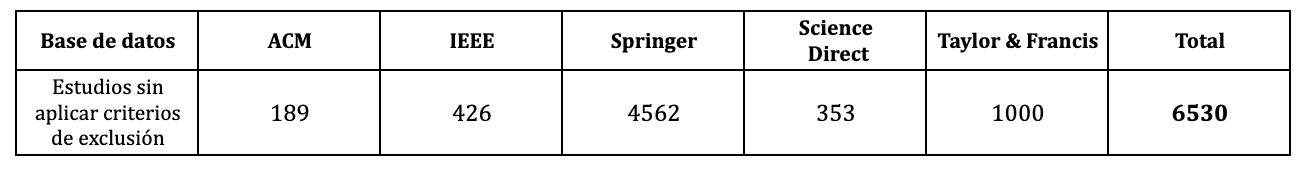
\includegraphics[width=\textwidth] {tablas-images/cp2/resumen-sin-criterios.png}
    \caption{Resumen de la búsqueda en bases de datos sin criterios de inclusión/exclusión}\label{tab:tabla-resumen-sin-criterios}
\end{table}
\begin{figure}[H]
    \centering
    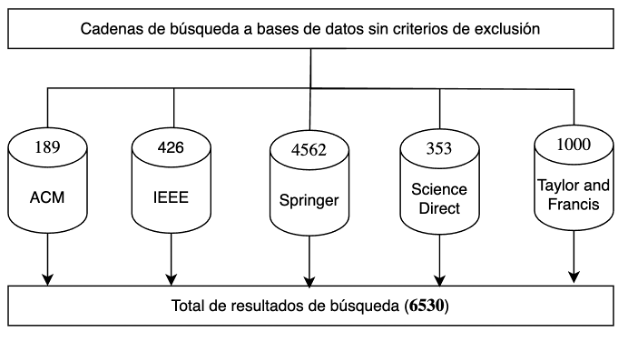
\includegraphics[scale=0.9]{tablas-images/cp2/bases-sin-criterio.png}
    \caption{Diagrama de búsqueda en bases de datos}\label{fig:tabla-resumen-busqueda}
\end{figure}

\subsubsection{Métricas de la búsqueda con criterios de inclusión/exclusión}\label{subsec:resumenBusquedaCriterios}
\noindent
Esta búsqueda se realizó considerando los criterios de exclusión e inclusión definidos previamente. Las cadena de búsqueda son exactamente iguales que antes, este punto se diferencia por la aplicación de filtros. Para ver las capturas de pantalla veáse el apéndice~\ref{sec:busqueda-con-criterios}.
La Tabla~\ref{tab:bases-sin-criterio} muestra los resultados obtenidos tras aplicar los criterios de inclusión y exclusión previamente definidos. A diferencia de la búsqueda inicial, en esta fase se utilizaron filtros específicos que redujeron significativamente la cantidad de publicaciones relevantes. En total se identificaron 976 documentos, distribuidos en las bases de datos de la siguiente manera: ACM (48), IEEE (134), Springer (592), Science Direct (46) y Taylor \& Francis (156).

\begin{table}[H]
\centering
\scriptsize
\setlength{\tabcolsep}{4pt}
\renewcommand{\arraystretch}{1.1}
\begin{tabular}{|l|c|c|c|c|c|c|}
\hline
\textbf{Bases de datos} & \textbf{ACM} & \textbf{IEEE} & \textbf{Springer} & \textbf{Science Direct} & \textbf{Taylor \& Francis} & \textbf{Total} \\
\hline
Con criterios aplicados & 48 & 134 & 592 & 46 & 156 & 976 \\
\hline
\end{tabular}
\caption{Resumen de la búsqueda en bases de datos con criterios de inclusión/exclusión}\label{tab:resumen-busqueda}
\end{table}
\begin{figure}[H]
    \centering
    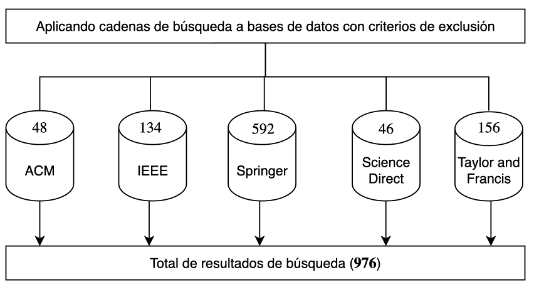
\includegraphics[width=\textwidth] {tablas-images/cp2/bases-con-criterio.png}
    \caption{Resumen de la búsqueda en bases de datos con criterios de inclusión/exclusión}\label{fig:tabla-resumen-busqueda-con-criterio}
\end{figure}

\section{Eliminación de duplicados}\label{sec:eliminacionDuplicados}
\noindent
La eliminación de duplicados se realizó haciendo uso de la herramienta de gestión de referencias Mendeley. Luego de obtener los artículos se agregaron a Mendeley y esta herramienta se encargó de eliminar duplicados. En este punto se eliminaron 274 artículos duplicados.

\section{Priorización de estudios}\label{sec:priorizacionEstudios}
\noindent
Luego de la selección inicial de los artículos, se procedió a revisar el \textit{title}, \textit{abstract} y \textit{keywords} de cada uno. Como resultado de esta revisión, se generaron métricas de calidad para cada artículo, con el fin de priorizar aquellos más relevantes para la investigación. Las métricas utilizadas fueron las siguientes:

\begin{itemize}
    \item \textbf{SCI} \textit{(Science Citation Index)}
    \item \textbf{CVI} \textit{(Core Value Index)}
    \item \textbf{IRRQ} \textit{(Index Relation Research Question)}
\end{itemize}
\noindent
Este proceso inició con un total de 771 artículos, los cuales fueron evaluados según su alineamiento con los objetivos de la investigación. La evaluación temática permitió identificar un total de 110 artículos con una relación directa con el enfoque planteado.

\section{Estrategia de búsqueda usando bola de nieve}\label{sec:bolaDeNieve}
\noindent
En esta etapa, se seleccionó el primer cuartil según el índice SCI, lo que resultó en un total de 24 artículos. Adicionalmente, se incluyó un artículo por criterio de inclusión directa, estableciendo así una línea base de 25 artículos. 
Partiendo de esta base, se aplicó la estrategia de bola de nieve en dos direcciones: hacia adelante y hacia atrás. Como resultado, se obtuvieron 87 artículos aplicando la técnica hacia atrás y 495 artículos aplicando la técnica hacia adelante.
Esto definió un nuevo conjunto de artículos para un proceso de selección adicional (\textit{screening}). En esta fase, se eliminaron 14 duplicados y 452 artículos fueron descartados por no aportar valor a la investigación.
Finalmente, se obtuvo un total de 116 artículos mediante esta estrategia de búsqueda.

\section{Diagrama de búsqueda}\label{sec:diagramaBusqueda}

\subsection{Usando cadenas de búsqueda}
\noindent
En el diagrama~\ref{tab:tabla-diagrama-cadena-busqueda} se puede apreciar la estrategia de búsqueda de artículos por medio de base de datos, aplicando las cadenas de búsqueda, se consolidaron los resultados de distintas bases de datos para obtener un total de 6530 resultados, posteriormente y aplicando criterios de exclusión se redujo esta cantidad a menos de 1000 resultados. Adicional a los criterios de exclusión, también se hizo eliminación de artículos duplicados, 205 por parte del ~\textit{Reference Manager}, y 69 por parte del ~\textit{SMS-Builder} para un total de 274 artículos removidos. Finalmente, se realiza la etapa de screening, donde se leen las secciones claves de los artículos, como ~\textit{abstract}, ~\textit{keywords} e introducción, a través de esto se pudo descargar 593 artículos que no eran pertinentes para el estudio.
\begin{table}[H]
    \centering
    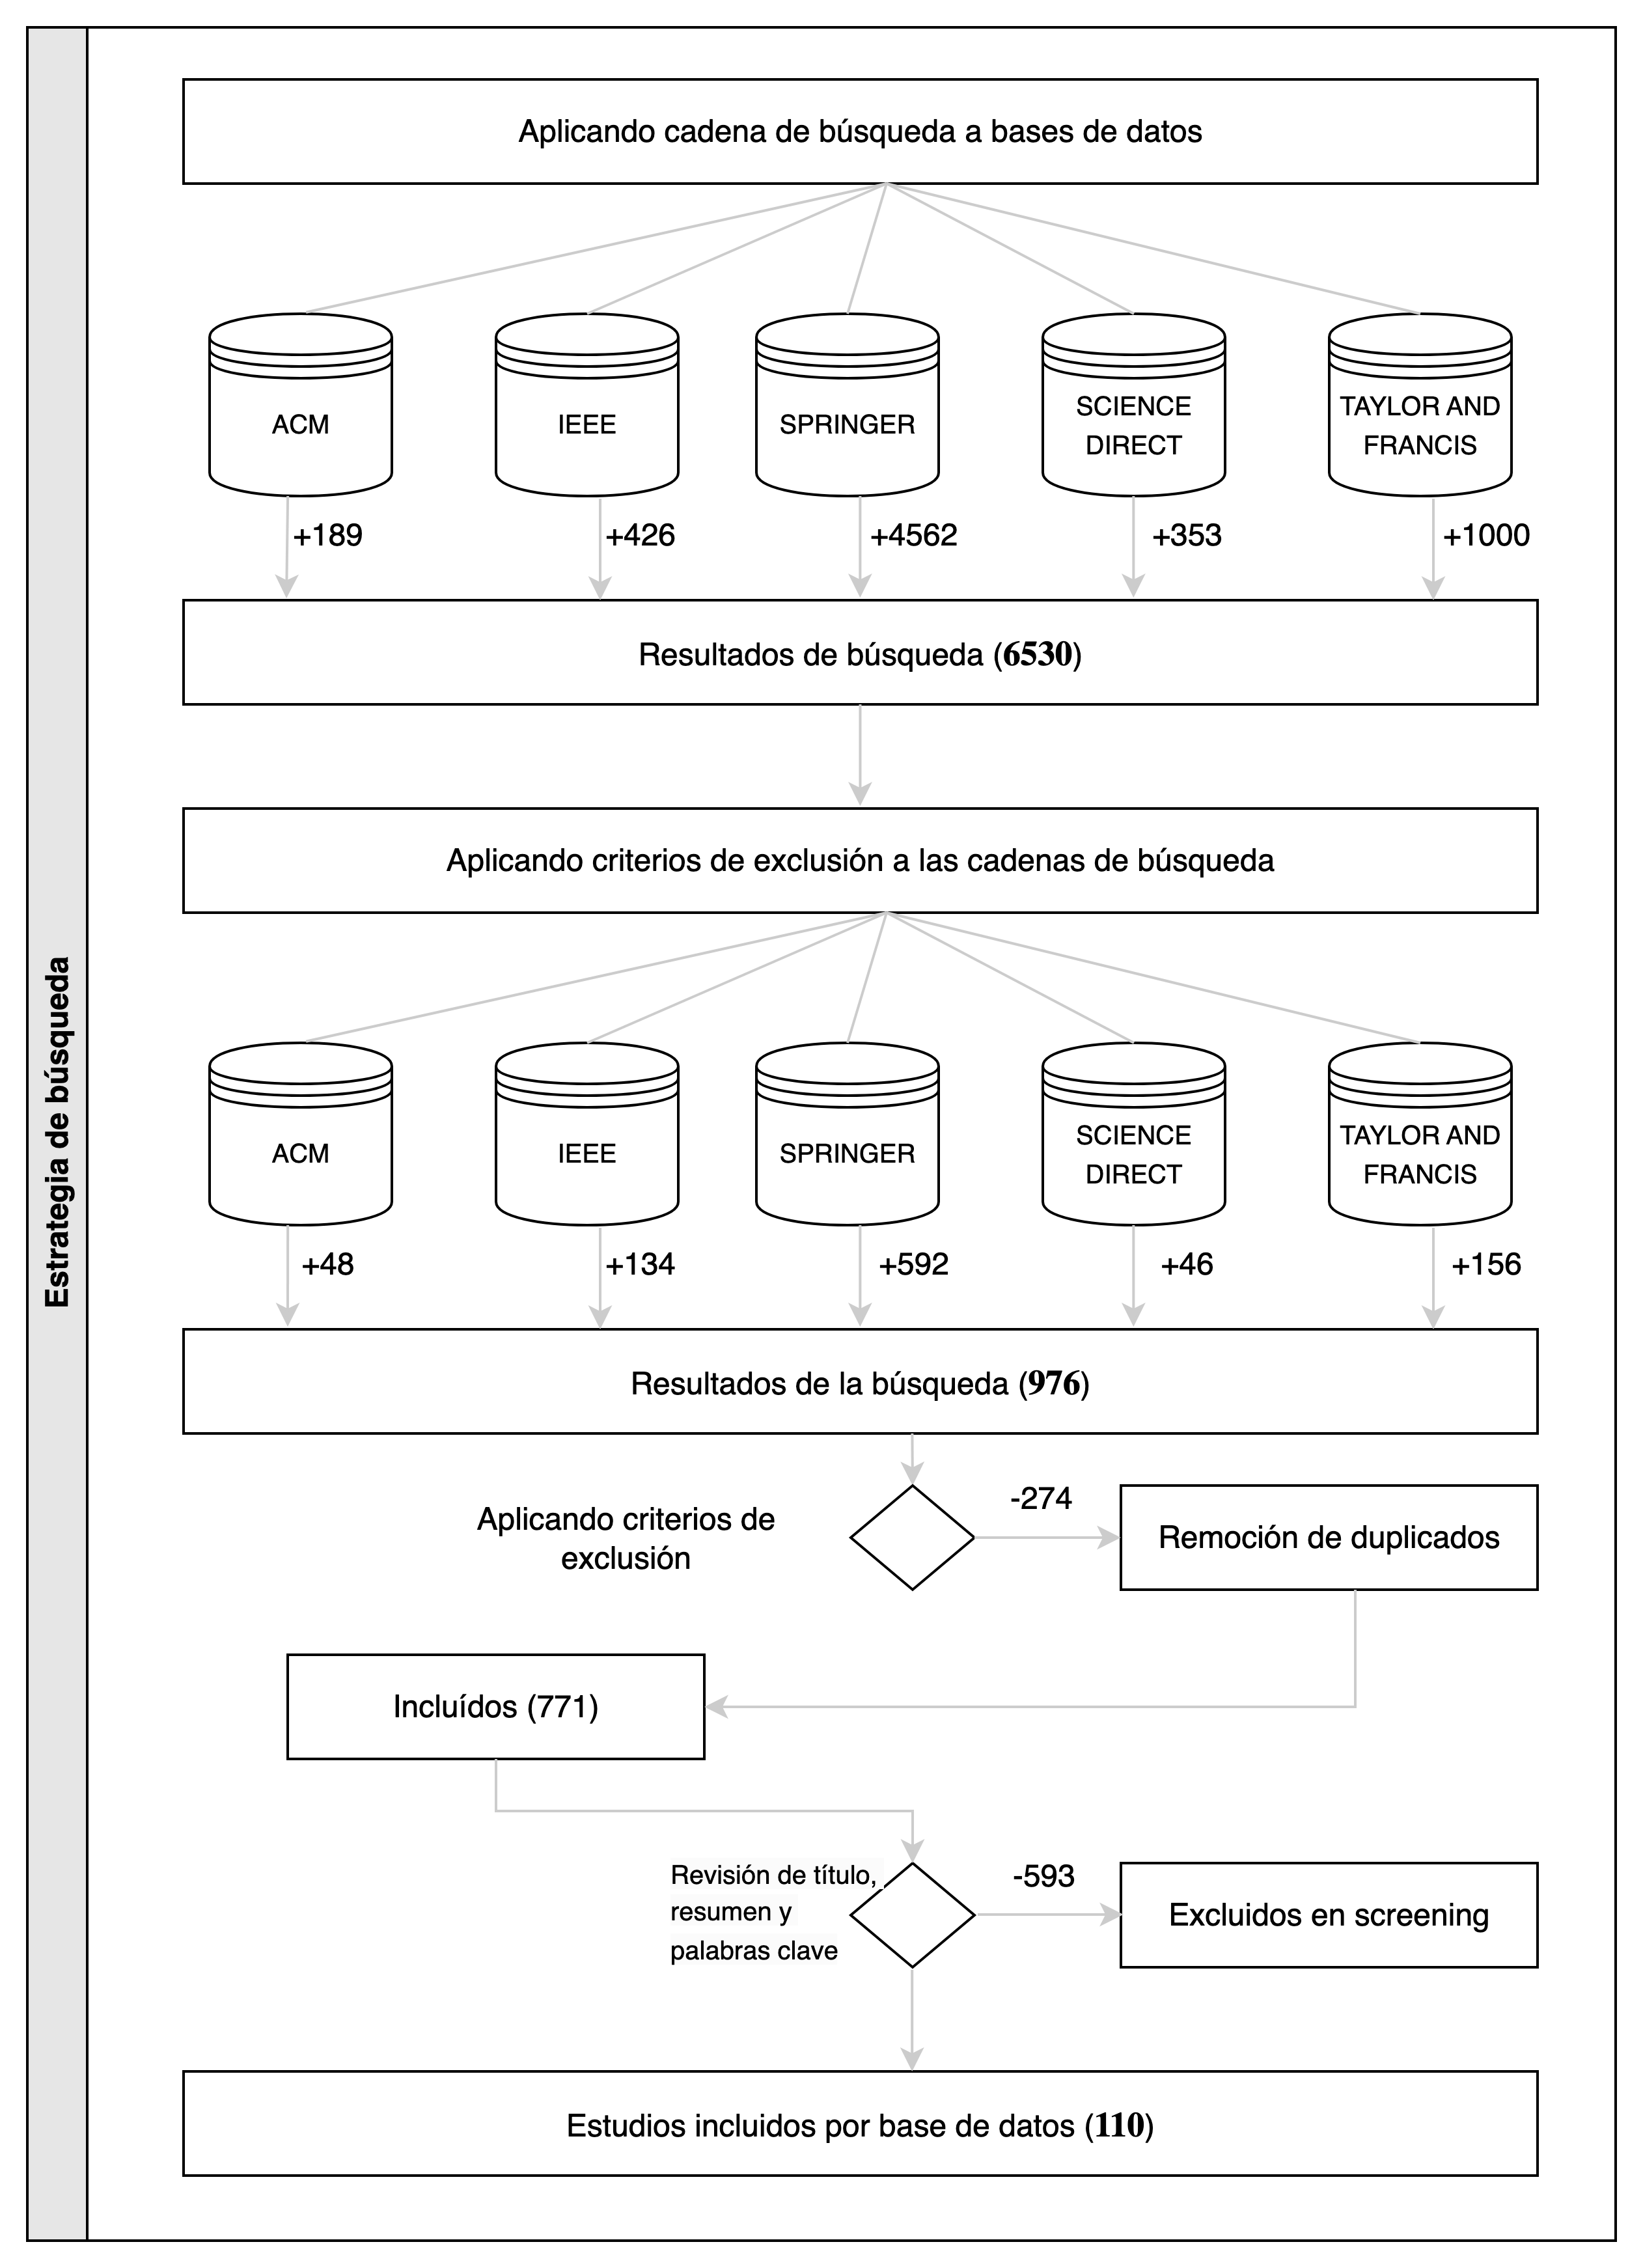
\includegraphics[scale=0.13]{tablas-images/cp2/diagrama-cadena-busqueda.png}
    \caption{Diagrama de la cadena de búsqueda}\label{tab:tabla-diagrama-cadena-busqueda}
\end{table}\label{img:busqueda-bd}

\subsection{Usando bola de nieve}
\noindent
Como segunda estrategia de búsqueda dentro del SMS, se aplicó la técnica de ~\textit{Snowball}, la cual consiste en extraer artículos adicionales a partir de las referencias citadas en los estudios obtenidos en la estrategia anterior y de los estudios que citan a estos. De los 110 estudios del paso anterior, se seleccionan aquellos que tenían un SCI más alto (primer cuartil) y se agrega uno por inclusión directa, con esto se obtiene un total de 25 artículos de línea base. Aplicando la técnica hacia adelante (artículos referenciados) se obtienen 87 nuevos estudios y la misma hacia atrás (artículos que referencian el artículo base) se obtienen 495, para un total de 582. Finalmente, se filtraron duplicados para iniciar la revisión del \textit{screening}. Como resultado 116 artículos fueron incluidos por bola de nieve. Todo este proceso se puede apreciar en la gráfica~\ref{tab:tabla-diagrama-bola-nieve-busqueda}.
\begin{table}[H]
    \centering
    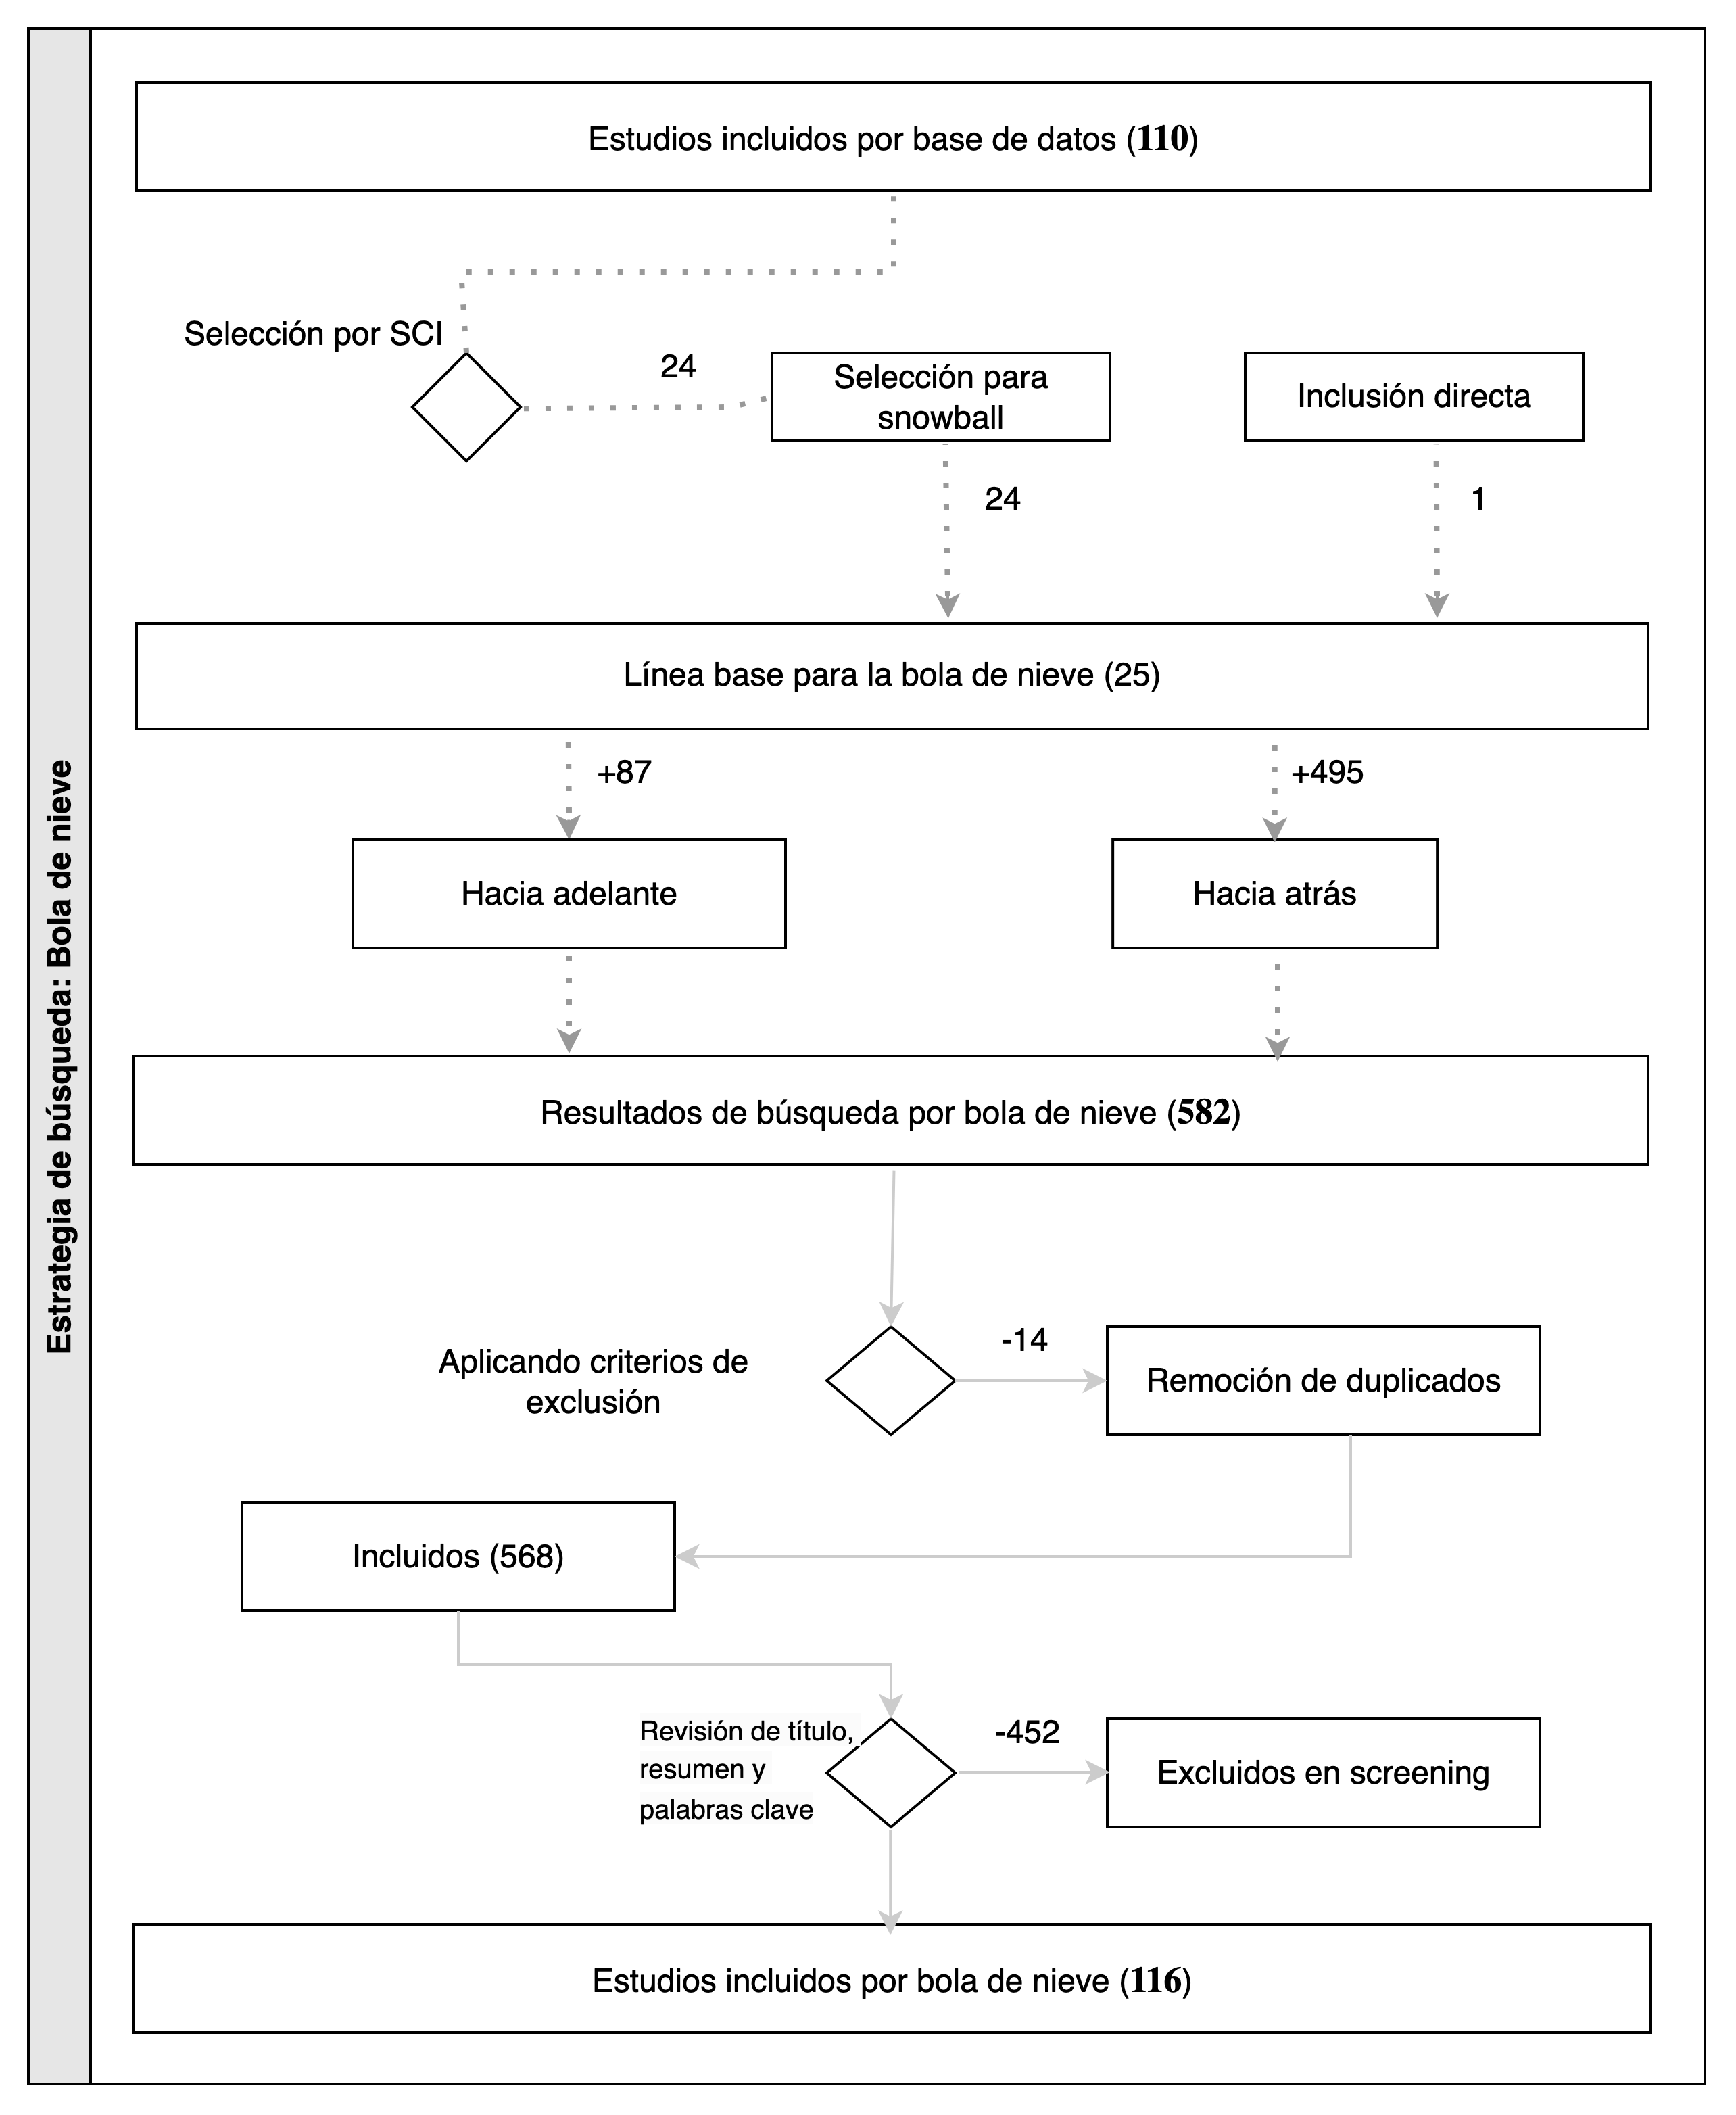
\includegraphics[scale=0.14]{tablas-images/cp2/diagrama-bola-nieve-busqueda.png}
    \caption{Diagrama de la búsqueda en bola de nieve}\label{tab:tabla-diagrama-bola-nieve-busqueda}
\end{table}

\section{Identificación de estudios}

\subsection{Artículos por año y métricas}
\noindent
A continuación se presentan las gráficas de los resultados de la búsqueda. 
\begin{figure}[H]
    \centering
    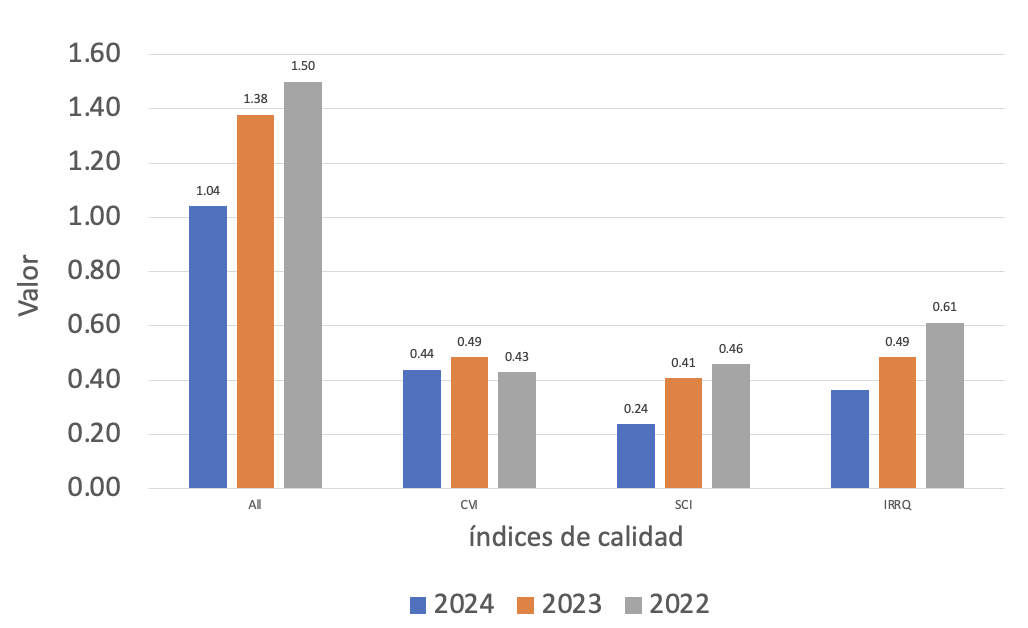
\includegraphics[width=\textwidth]{tablas-images/cp2/diagrama-articulos-ano-metrica.png}
    \caption{Artículos por métricas y año}\label{fig:diagrama-articulos-ano-metrica}
\end{figure}

\begin{figure}[H]
    \centering
    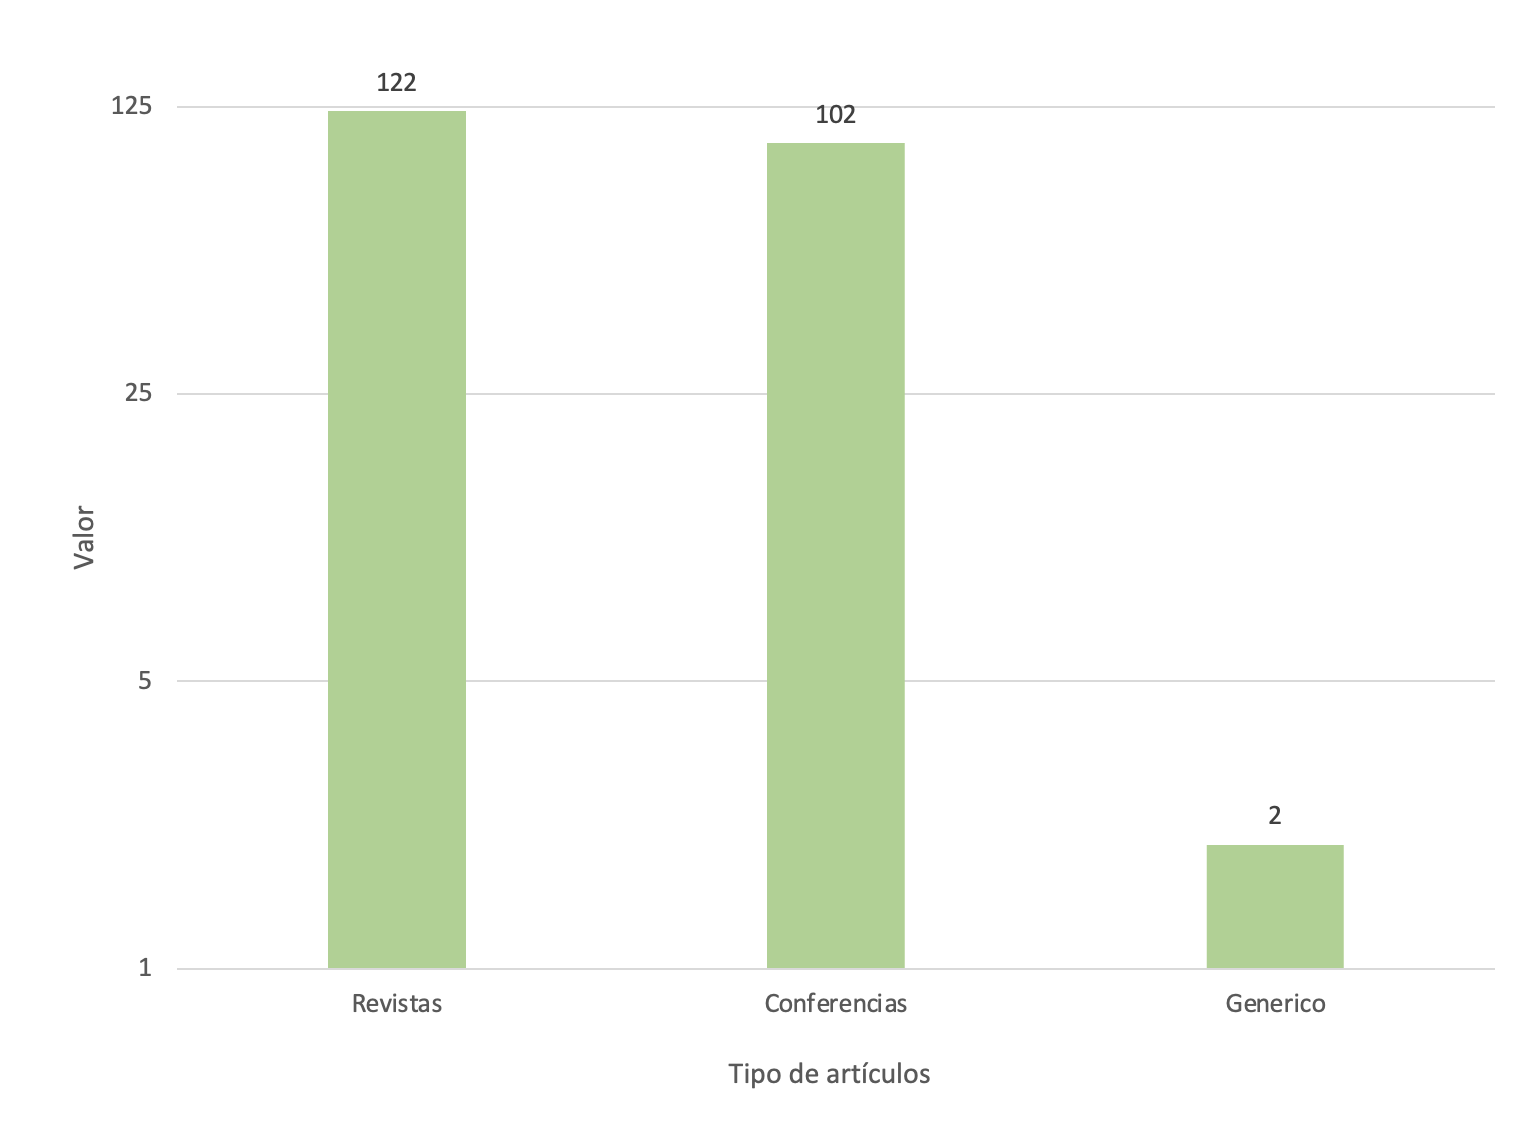
\includegraphics[width=\textwidth]{tablas-images/cp2/tipos-articulos.png}
    \caption{Artículos por tipo}\label{fig:tipos-articulos}
\end{figure}

\begin{figure}[H]
    \centering
    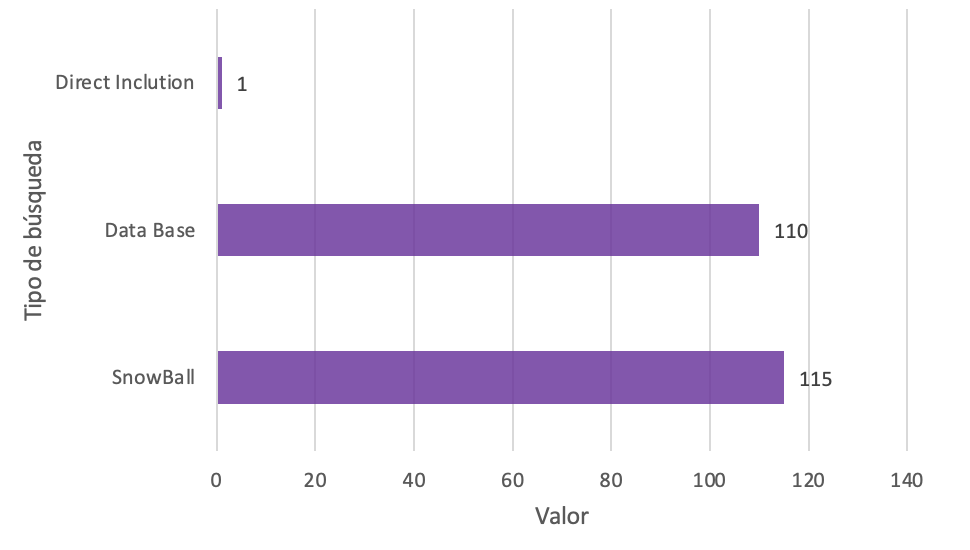
\includegraphics[width=\textwidth]{tablas-images/cp2/estrategia-busqueda-articulos.png}
    \caption{Estrategia de búsqueda de artículos}\label{fig:estrategia-busqueda-articulos}
\end{figure}

\begin{figure}[H]
    \centering
    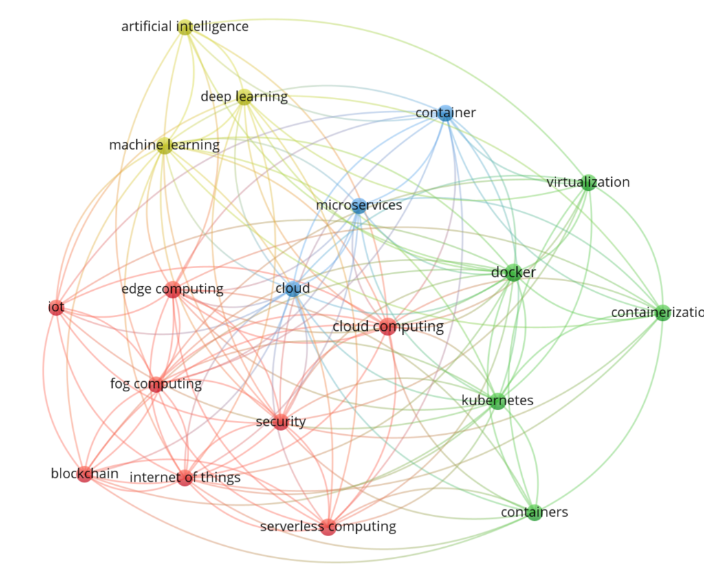
\includegraphics[width=\textwidth]{tablas-images/cp2/diagrama-red-busqueda.png}
    \caption{Diagrama de red de los artículos}\label{fig:diagrama-red-articulos}
\end{figure}

\section{Información de la herramienta}

\noindent
La herramienta utilizada para este proceso de revisión de la literatura fue \textbf{SMS-BUILDER}, la cual se encuentra disponible en \textit{Docker Hub}. La imagen puede consultarse en el siguiente enlace:

\begin{center}
\href{https://hub.docker.com/r/griduq/sms-builder}{\texttt{https://hub.docker.com/r/griduq/sms-builder}}
\end{center}

\section{Reproducibilidad del método}
\noindent
Con el fin de fomentar la reproducibilidad del método de revisión, se proporcionan dos mecanismos de verificación que permiten a los revisores y lectores acceder de forma transparente a la información utilizada, generada mediante la herramienta SMS-Builder de~\cite{SMSBuilder2020}
\begin{itemize}
  \item Un enlace de acceso público a la instancia de SMS-Builder que contiene todos los datos del proceso de revisión sistemática: \href{https://sms-vbc.iti.grid.uniquindio.edu.co/sms.xhtml}{link}. Las credenciales de acceso son ``invitado'' tanto para el nombre de usuario como para la contraseña.
  \item Una imagen de Docker de acceso público que integra toda la documentación necesaria para crear un contenedor con los datos del proceso: \href{https://hub.docker.com/r/anubis1001/tg-vbc-sms-builder}{link}.
\end{itemize}

\noindent
Adicionalmente, se implementaron procesos de respaldo como medida de seguridad. Estos \textit{backups} fueron almacenados en ubicaciones diferentes, siguiendo la estrategia de respaldo \textbf{3--2--1}.

\section{Conclusiones de la revisión sistemática de la literatura}
\noindent
Esta sección presenta un mapeo sistemático de la literatura sobre tecnologías de virtualización basadas en contenedores, principalmente relacionada con la educación, la investigación y la extensión. Dentro del \SMS, se definió un esquema de clasificación según los temas específicos establecidos durante la fase de planificación. Este esquema proporciona un mapeo de la información en tablas y gráficos estadísticos que ayudan a describir los datos y su relación con las preguntas de investigación. El mapeo sistemático reveló una creciente proliferación de estudios relacionados con las tecnologías de \VBC, incluyendo estudios en diferentes áreas y aplicaciones. Esta proliferación de estudios podría ser contraproducente para ciertas partes interesadas a la hora de implementar arquitecturas con estas tecnologías. Además, puede provocar una saturación de la literatura y dificultar el desarrollo, principalmente debido al abrumador volumen de información disponible. Más allá de los resultados obtenidos en este \SMS, los estudios se analizaron explorando la información subyacente y las tendencias. De este modo, se identificó una creciente adopción de la virtualización ligera en la implementación de soluciones, con especial énfasis en la computación en la nube y orquestadores como Kubernetes. Este liderazgo se ve reforzado por la necesidad de las organizaciones de proporcionar redundancia, fiabilidad y escalabilidad en sus aplicaciones y servicios.